% ============================================================
%  SESSION 1 — Web + HTML + CSS (Temel)
%  XeLaTeX ile derleyin: xelatex session-01.tex
% ============================================================
\documentclass[12pt, a4paper]{article}

% ---------- Font & Dil ----------
\usepackage{fontspec}
\usepackage[turkish, shorthands=off]{babel}
\setmainfont{Georgia}
\setsansfont{Arial}
\setmonofont{Courier New}

% ---------- Sayfa Düzeni ----------
\usepackage[top=2.2cm, bottom=2.2cm, left=2.4cm, right=2.4cm]{geometry}
\usepackage{parskip}
\setlength{\parindent}{0pt}

% ---------- Renkler ----------
\usepackage{xcolor}
\definecolor{primary}{HTML}{2563EB}
\definecolor{secondary}{HTML}{7C3AED}
\definecolor{accent}{HTML}{059669}
\definecolor{warning}{HTML}{D97706}
\definecolor{danger}{HTML}{DC2626}
\definecolor{lightbg}{HTML}{F1F5F9}
\definecolor{codebg}{HTML}{1E293B}
\definecolor{codefg}{HTML}{E2E8F0}
\definecolor{htmlcol}{HTML}{E34C26}
\definecolor{csscol}{HTML}{264DE4}
\definecolor{blockcolor}{HTML}{3B82F6}
\definecolor{inlinecolor}{HTML}{8B5CF6}
\definecolor{flexcolor}{HTML}{10B981}

% ---------- Kutular (tcolorbox) ----------
\usepackage[skins, breakable, listings]{tcolorbox}
\tcbuselibrary{skins, breakable, listings}

\newtcolorbox{infobox}[1][]{
  enhanced, breakable,
  colback=primary!8, colframe=primary,
  fonttitle=\bfseries\sffamily,
  title={#1},
  left=6pt, right=6pt, top=4pt, bottom=4pt,
  arc=4pt
}

\newtcolorbox{warningbox}[1][]{
  enhanced, breakable,
  colback=warning!10, colframe=warning,
  fonttitle=\bfseries\sffamily,
  title={#1},
  left=6pt, right=6pt, top=4pt, bottom=4pt,
  arc=4pt
}

\newtcolorbox{practicebox}[1][]{
  enhanced, breakable,
  colback=accent!8, colframe=accent,
  fonttitle=\bfseries\sffamily,
  title={#1},
  left=6pt, right=6pt, top=4pt, bottom=4pt,
  arc=4pt
}

\newtcolorbox{definebox}[1][]{
  enhanced, breakable,
  colback=secondary!7, colframe=secondary,
  fonttitle=\bfseries\sffamily,
  title={#1},
  left=6pt, right=6pt, top=4pt, bottom=4pt,
  arc=4pt
}

% ---------- Kod Listeleme ----------
\usepackage{listings}

% Türkçe karakterleri listings içinde doğru göstermek için literate map
\lstset{literate=
  {ı}{{\texttt{ı}}}1  {İ}{{\texttt{İ}}}1
  {ğ}{{\texttt{ğ}}}1  {Ğ}{{\texttt{Ğ}}}1
  {ş}{{\texttt{ş}}}1  {Ş}{{\texttt{Ş}}}1
  {ü}{{\texttt{ü}}}1  {Ü}{{\texttt{Ü}}}1
  {ö}{{\texttt{ö}}}1  {Ö}{{\texttt{Ö}}}1
  {ç}{{\texttt{ç}}}1  {Ç}{{\texttt{Ç}}}1
}

\lstdefinestyle{htmlstyle}{
  backgroundcolor=\color{codebg},
  basicstyle=\ttfamily\small\color{codefg},
  keywordstyle=\color{htmlcol}\bfseries,
  stringstyle=\color{accent},
  commentstyle=\color{gray}\itshape,
  morekeywords={DOCTYPE,html,head,body,title,h1,h2,h3,p,div,span,
    nav,main,section,article,header,footer,aside,ul,ol,li,
    form,input,button,label,a,img,meta,link,type,id,name,
    placeholder,href,class,charset,lang,for,src,alt,rel},
  morestring=[b]",
  morecomment=[s]{<!--}{-->},
  showstringspaces=false,
  breaklines=true,
  frame=none,
  xleftmargin=8pt, xrightmargin=8pt,
}

\lstdefinestyle{cssstyle}{
  backgroundcolor=\color{codebg},
  basicstyle=\ttfamily\small\color{codefg},
  keywordstyle=\color{csscol!70!white}\bfseries,
  stringstyle=\color{accent},
  commentstyle=\color{gray}\itshape,
  morekeywords={display,flex,justify-content,align-items,flex-direction,
    margin,padding,border,background,background-color,color,font-size,
    font-weight,font-family,width,height,box-sizing,border-box,center,
    space-between,space-around,flex-start,flex-end,block,inline,
    inline-block,none,row,column,gap,border-radius,box-shadow,
    overflow,hidden,text-align,transition,ease,transform,translateY,
    cursor,pointer,sans-serif,white,solid,flex-wrap,wrap,nowrap,flex,
    rgba,stretch,line-height},
  morecomment=[l]{//},
  morecomment=[s]{/*}{*/},
  showstringspaces=false,
  breaklines=true,
  frame=none,
  xleftmargin=8pt, xrightmargin=8pt,
}

% ---------- Grafikler ----------
\usepackage{graphicx}
\usepackage{caption}
\usepackage{tikz}
\usetikzlibrary{arrows.meta, shapes.geometric, positioning, calc}

% ---------- Tablo ----------
\usepackage{booktabs}
\usepackage{tabularx}
\usepackage{array}

% ---------- Başlık Stilleri ----------
\makeatletter
\renewcommand{\section}{%
  \@startsection{section}{1}{\z@}%
    {-1.5ex plus -1ex minus -0.5ex}%
    {0.8ex plus 0.3ex}%
    {\normalfont\Large\bfseries\sffamily\color{primary}}%
}
\renewcommand{\subsection}{%
  \@startsection{subsection}{2}{\z@}%
    {-1.2ex plus -0.8ex minus -0.4ex}%
    {0.5ex plus 0.2ex}%
    {\normalfont\large\bfseries\sffamily\color{secondary}}%
}
\renewcommand{\subsubsection}{%
  \@startsection{subsubsection}{3}{\z@}%
    {-1ex plus -0.6ex minus -0.3ex}%
    {0.4ex}%
    {\normalfont\normalsize\bfseries\sffamily\color{accent}}%
}
\makeatother

% ---------- Üstbilgi / Altbilgi ----------
\usepackage{fancyhdr}
\pagestyle{fancy}
\fancyhf{}
\fancyhead[L]{\small\sffamily\color{gray} Front-end + Next.js Eğitimi}
\fancyhead[R]{\small\sffamily\color{gray} Session 1 — Web + HTML + CSS (Temel)}
\fancyfoot[C]{\small\sffamily\color{gray} \thepage}
\renewcommand{\headrulewidth}{0.4pt}

% ---------- Diğer ----------
\usepackage{enumitem}
\setlist[itemize]{leftmargin=1.5em, itemsep=2pt}
\setlist[enumerate]{leftmargin=1.5em, itemsep=2pt}
\usepackage{hyperref}
\hypersetup{colorlinks=true, linkcolor=primary, urlcolor=primary}
\usepackage{fontawesome5}

% ---------- Yardımcı Komut ----------
\newcommand{\timebadge}[1]{%
  \noindent
  \colorbox{primary}{\color{white}\sffamily\bfseries\small\strut~~\faStopwatch~~#1~~}%
  \par\vspace{4pt}%
}

% ============================================================
\begin{document}

% ============================================================
%  KAPAK
% ============================================================
\thispagestyle{empty}

\begin{tikzpicture}[remember picture, overlay]
  \fill[primary] (current page.north west)
    rectangle ++(\paperwidth, -8.0cm);
  \fill[secondary] (current page.north west) ++(0,-7.8cm)
    rectangle ++(\paperwidth, -0.28cm);
\end{tikzpicture}

\vspace*{1.6cm}
{\color{white}\sffamily
  \hspace{1.2cm}{\small SESSION 1 / 8 \quad|\quad 27 Nisan 2026 \quad|\quad~90 dakika}\\[12pt]
  \hspace{1.2cm}{\fontsize{30}{36}\selectfont\bfseries Web + HTML + CSS}\\[8pt]
  \hspace{1.2cm}{\Large Temel Kavramlar ve İlk UI}
}

\vspace{0.9cm}

\vspace{0.1cm}

\begin{tcolorbox}[enhanced,
  colback=lightbg, colframe=gray!30, arc=4pt,
  title={\sffamily\bfseries\color{primary}\faStream\quad Session Akışı},
  fonttitle=\bfseries\sffamily]
\sffamily\small
\begin{tabularx}{\textwidth}{>{\bfseries\color{primary}}l X l}
\toprule
Süre & Konu & Anahtar Kavramlar \\
\midrule
0--15 dk  & Web Nasıl Çalışır?              & Browser, Server, HTTP, Request/Response \\
15--35 dk & HTML Temelleri                  & Etiketler, Semantic HTML, Form öğeleri \\
35--70 dk & CSS Temelleri                   & Box Model, Display, Flexbox \\
70--90 dk & \textcolor{accent}{Pratik: Card UI} & Flex layout, gerçek bileşen \\
\bottomrule
\end{tabularx}
\end{tcolorbox}

% ============================================================
\clearpage
\section{\faGlobe\ Web Nasıl Çalışır?}
\timebadge{0--15 dakika}

\subsection{Browser -- Server İlişkisi}

Web uygulamaları iki taraf arasındaki bir iletişimdir:

\vspace{8pt}
\begin{center}
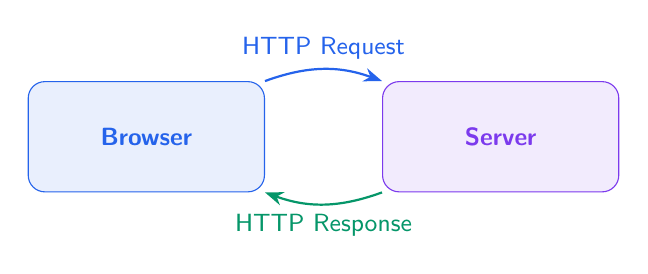
\begin{tikzpicture}[node distance=4.5cm, >=Stealth]
  \node[draw=primary, fill=primary!10, rounded corners=6pt,
        minimum width=3cm, minimum height=1.4cm,
        font=\sffamily\bfseries\small, text=primary] (browser)
        {Browser};

  \node[draw=secondary, fill=secondary!10, rounded corners=6pt,
        minimum width=3cm, minimum height=1.4cm,
        font=\sffamily\bfseries\small, text=secondary,
        right of=browser] (server)
        {Server};

  \draw[->, thick, color=primary, bend left=20]
    (browser.north east) to
    node[above, font=\small\sffamily, text=primary] {HTTP Request}
    (server.north west);

  \draw[->, thick, color=accent, bend left=20]
    (server.south west) to
    node[below, font=\small\sffamily, text=accent] {HTTP Response}
    (browser.south east);
\end{tikzpicture}
\end{center}

\begin{definebox}[Temel Kavramlar]
\begin{itemize}
  \item \textbf{Browser (Tarayıcı):} Chrome, Firefox, Safari. HTML/CSS/JS'i okuyup ekrana çizer.
  \item \textbf{Server (Sunucu):} İstekleri alan, cevap dönen bilgisayar/servis.
  \item \textbf{HTTP:} İkisi arasındaki konuşma dili (protokol).
  \item \textbf{URL:} Kaynak adresi --- \texttt{https://ornek.com/sayfa}
\end{itemize}
\end{definebox}

\subsection{Request / Response Döngüsü}

\begin{enumerate}
  \item Kullanıcı adres çubuğuna URL yazar ve Enter'a basar.
  \item Browser sunucuya \textbf{HTTP Request} gönderir.
  \item Sunucu isteği işler ve \textbf{HTTP Response} döner (HTML dosyası vb.).
  \item Browser aldığı HTML'i okur, CSS ile renklendirir, JS ile canlandırır.
\end{enumerate}

\subsection{HTML -- CSS -- JS Akışı}

\begin{center}
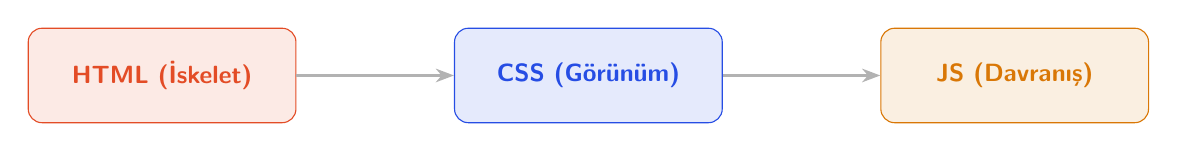
\begin{tikzpicture}[node distance=0.4cm, >=Stealth]
  \node[draw=htmlcol, fill=htmlcol!12, rounded corners=5pt,
        minimum width=3.4cm, minimum height=1.2cm,
        font=\sffamily\bfseries\small\color{htmlcol}] (html)
        {HTML (İskelet)};

  \node[draw=csscol, fill=csscol!12, rounded corners=5pt,
        minimum width=3.4cm, minimum height=1.2cm,
        font=\sffamily\bfseries\small\color{csscol},
        right=2cm of html] (css)
        {CSS (Görünüm)};

  \node[draw=warning, fill=warning!12, rounded corners=5pt,
        minimum width=3.4cm, minimum height=1.2cm,
        font=\sffamily\bfseries\small\color{warning},
        right=2cm of css] (js)
        {JS (Davranış)};

  \draw[->, thick, color=gray!60] (html) -- (css);
  \draw[->, thick, color=gray!60] (css)  -- (js);
\end{tikzpicture}
\end{center}

\begin{infobox}[\faLightbulb\ Analoji]
Bir binanın \textbf{iskeleti} HTML, \textbf{boyası ve dekorasyonu} CSS,
\textbf{asansörü ve otomatik kapıları} JavaScript'tir.
\end{infobox}

% ============================================================
\newpage
\section{\faCode\ HTML Temelleri}
\timebadge{15--35 dakika}

\subsection{Temel Yapı}

\begin{tcolorbox}[enhanced, colback=codebg, colframe=gray!30,
    colbacktitle=primary!85!black, coltitle=white, arc=4pt,
    title={\sffamily\bfseries\small Minimal HTML Belgesi}]
\begin{lstlisting}[style=htmlstyle]
<!DOCTYPE html>
<html lang="tr">
  <head>
    <meta charset="UTF-8" />
    <meta name="viewport" content="width=device-width, initial-scale=1.0" />
    <title>My Page</title>
  </head>
  <body>
    <h1>Hello World!</h1>
    <p>My first HTML page.</p>
  </body>
</html>
\end{lstlisting}
\end{tcolorbox}

\begin{warningbox}[\faExclamationTriangle\ Dikkat]
Her açılan etiketin kapatılması gerekir: \texttt{<p>} açılır,
\texttt{</p>} kapatılır. Bazı etiketler self-closing'dir:
\texttt{<meta />}, \texttt{<img />}, \texttt{<input />}
\end{warningbox}

\subsection{Semantic (Anlamlı) Etiketler}

Semantic etiketler içeriğin \textit{ne olduğunu} söyler; okunabilirlik ve SEO'yu iyileştirir.

\vspace{6pt}
\begin{tabularx}{\textwidth}{>{\ttfamily\color{primary}}l X}
\toprule
\normalfont\bfseries Etiket & \normalfont\bfseries Anlamı \\
\midrule
<header>   & Sayfa veya bölüm başlığı \\
<nav>      & Navigasyon/menü alanı \\
<main>     & Sayfanın ana içeriği (sayfa başına 1 tane) \\
<section>  & Tematik bir içerik bölümü \\
<article>  & Bağımsız, paylaşılabilir içerik (blog yazısı vb.) \\
<aside>    & Yan bilgi, kenar çubuğu \\
<footer>   & Sayfa veya bölüm altlığı \\
\bottomrule
\end{tabularx}

\vspace{8pt}

\begin{tcolorbox}[enhanced, colback=codebg, colframe=gray!30,
    colbacktitle=primary!85!black, coltitle=white, arc=4pt,
    title={\sffamily\bfseries\small Semantic Layout Örneği}]
\begin{lstlisting}[style=htmlstyle]
<body>
  <header>
    <nav>
      <a href="/">Home</a>
      <a href="/about">About</a>
    </nav>
  </header>

  <main>
    <section>
      <h2>Featured Products</h2>
      <article>
        <h3>Product Name</h3>
        <p>Description text...</p>
      </article>
    </section>
  </main>

  <footer>
    <p>2026 Company Name</p>
  </footer>
</body>
\end{lstlisting}
\end{tcolorbox}

\subsection{Form Elementleri}

\begin{tcolorbox}[enhanced, colback=codebg, colframe=gray!30,
    colbacktitle=primary!85!black, coltitle=white, arc=4pt,
    title={\sffamily\bfseries\small Form Örneği}]
\begin{lstlisting}[style=htmlstyle]
<form>
  <!-- Text input -->
  <label for="fullName">Full name:</label>
  <input type="text" id="fullName" name="fullName" placeholder="Enter your name" />

  <!-- Email -->
  <label for="email">Email:</label>
  <input type="email" id="email" name="email" />

  <!-- Buttons -->
  <button type="submit">Submit</button>
  <button type="button">Cancel</button>
</form>
\end{lstlisting}
\end{tcolorbox}

\begin{infobox}[\faLightbulb\ \texttt{label} + \texttt{id} bağlantısı]
\texttt{<label for="ad">} ile \texttt{<input id="ad">} eşleşince,
etikete tıklamak imleci input'a taşır --- erişilebilirlik için kritiktir.
\end{infobox}

% ============================================================
\newpage
\section{\faPaintBrush\ CSS Temelleri}
\timebadge{35--70 dakika}

\subsection{CSS Nasıl Bağlanır?}

\begin{tcolorbox}[enhanced, colback=codebg, colframe=gray!30,
    colbacktitle=primary!85!black, coltitle=white, arc=4pt,
    title={\sffamily\bfseries\small CSS Bağlama Yöntemleri}]
\begin{lstlisting}[style=htmlstyle]
<!-- 1. External file (recommended) -->
<link rel="stylesheet" href="style.css" />

<!-- 2. Internal <style> tag -->
<style>
  body { margin: 0; }
</style>

<!-- 3. Inline style (avoid) -->
<p style="color: red;">Text</p>
\end{lstlisting}
\end{tcolorbox}

% ----------------------------------------------------------
\subsection{Box Model}

Her HTML elemanı aslında bir \textbf{kutu}dur ve dört katmandan oluşur:

\vspace{8pt}
\begin{center}
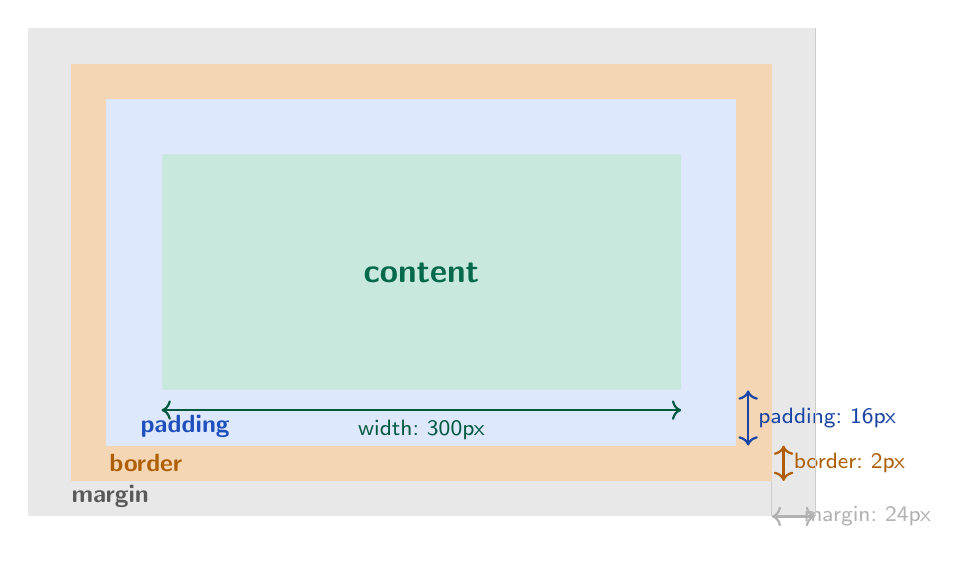
\begin{tikzpicture}
  % margin (en dış)
  \fill[gray!18]    (0,0)       rectangle (10, 6.2);
  % border
  \fill[warning!30] (0.55,0.45) rectangle (9.45, 5.75);
  % padding
  \fill[primary!15] (1.0, 0.9)  rectangle (9.0, 5.3);
  % content
  \fill[accent!22]  (1.7, 1.6)  rectangle (8.3, 4.6);

  % Katman etiketleri
  \node[gray!70!black, font=\sffamily\bfseries\small]
    at (1.05, 0.25) {margin};
  \node[warning!80!black, font=\sffamily\bfseries\small]
    at (1.5, 0.68) {border};
  \node[primary!80!black, font=\sffamily\bfseries\small]
    at (2.0, 1.15) {padding};
  \node[accent!70!black, font=\sffamily\bfseries\large]
    at (5.0, 3.1)  {content};

  % Boyut okları — yatay (content genişliği)
  \draw[<->, thick, accent!60!black]
    (1.7, 1.35) -- node[below, font=\sffamily\footnotesize] {width: 300px} (8.3, 1.35);

  % Boyut okları — dikey (padding)
  \draw[<->, thick, primary!70!black]
    (9.15, 0.9) -- node[right, font=\sffamily\footnotesize] {padding: 16px} (9.15, 1.6);

  % Boyut okları — border
  \draw[<->, thick, warning!80!black]
    (9.6, 0.45) -- node[right, font=\sffamily\footnotesize] {border: 2px} (9.6, 0.9);

  % Boyut okları — margin (sağ)
  \draw[<->, thick, gray!60]
    (9.45, 0.0) -- node[right, font=\sffamily\footnotesize] {margin: 24px} (10, 0.0);
  \draw[gray!40] (9.45, 0.0) -- (9.45, 0.45);
  \draw[gray!40] (10.0, 0.0) -- (10.0, 6.2);
\end{tikzpicture}
\end{center}

\begin{tcolorbox}[enhanced, colback=codebg, colframe=gray!30,
    colbacktitle=primary!85!black, coltitle=white, arc=4pt]
\begin{lstlisting}[style=cssstyle]
.kutu {
  width: 300px;            /* content width               */
  padding: 16px;           /* inner space (all 4 sides)   */
  border: 2px solid #ccc;  /* border width                */
  margin: 24px;            /* outer space (all 4 sides)   */

  /* padding + border included in total width */
  box-sizing: border-box;
}
\end{lstlisting}
\end{tcolorbox}

% ----------------------------------------------------------
\newpage
\subsection{Display Özellikleri}

\texttt{display} özelliği, bir elemanın sayfada nasıl konumlandırılacağını belirler.

\vspace{10pt}

% ---- display: block görsel ----
\begin{tcolorbox}[enhanced, colback=blockcolor!6, colframe=blockcolor,
    title={\sffamily\bfseries\color{blockcolor} display: block},
    fonttitle=\bfseries\sffamily, arc=4pt,
    left=6pt, right=6pt, top=4pt, bottom=4pt]
\begin{minipage}{0.46\textwidth}
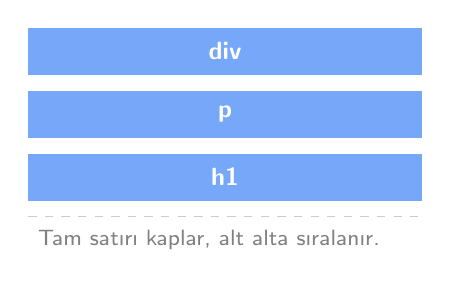
\begin{tikzpicture}
  \fill[blockcolor!70] (0,2.4) rectangle (5.0, 3.0);
  \fill[blockcolor!70] (0,1.6) rectangle (5.0, 2.2);
  \fill[blockcolor!70] (0,0.8) rectangle (5.0, 1.4);
  \node[white, font=\sffamily\small\bfseries] at (2.5, 2.7) {div};
  \node[white, font=\sffamily\small\bfseries] at (2.5, 1.9) {p};
  \node[white, font=\sffamily\small\bfseries] at (2.5, 1.1) {h1};
  \draw[gray!40, dashed] (0,0.6) -- (5.0,0.6);
  \node[gray, font=\sffamily\footnotesize, right] at (0, 0.3) {Tam satırı kaplar, alt alta sıralanır.};
\end{tikzpicture}
\end{minipage}
\hfill
\begin{minipage}{0.50\textwidth}
\begin{lstlisting}[style=cssstyle, basicstyle=\ttfamily\footnotesize\color{codefg}]
div, p, h1, h2, section,
article, header, footer {
  display: block; /* default */
}
\end{lstlisting}
\end{minipage}
\end{tcolorbox}

\vspace{6pt}

% ---- display: inline görsel ----
\begin{tcolorbox}[enhanced, colback=inlinecolor!6, colframe=inlinecolor,
    title={\sffamily\bfseries\color{inlinecolor} display: inline},
    fonttitle=\bfseries\sffamily, arc=4pt,
    left=6pt, right=6pt, top=4pt, bottom=4pt]
\begin{minipage}{0.46\textwidth}
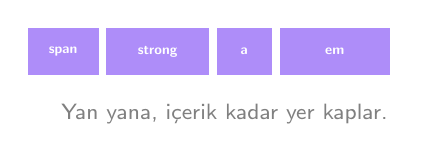
\begin{tikzpicture}
  \fill[inlinecolor!70] (0.0,0.8) rectangle (0.9,1.4);
  \fill[inlinecolor!70] (1.0,0.8) rectangle (2.3,1.4);
  \fill[inlinecolor!70] (2.4,0.8) rectangle (3.1,1.4);
  \fill[inlinecolor!70] (3.2,0.8) rectangle (4.6,1.4);
  \node[white, font=\sffamily\tiny\bfseries] at (0.45,1.1) {span};
  \node[white, font=\sffamily\tiny\bfseries] at (1.65,1.1) {strong};
  \node[white, font=\sffamily\tiny\bfseries] at (2.75,1.1) {a};
  \node[white, font=\sffamily\tiny\bfseries] at (3.9, 1.1) {em};
  \node[gray, font=\sffamily\footnotesize] at (2.5, 0.3) {Yan yana, içerik kadar yer kaplar.};
\end{tikzpicture}
\end{minipage}
\hfill
\begin{minipage}{0.50\textwidth}
\begin{lstlisting}[style=cssstyle, basicstyle=\ttfamily\footnotesize\color{codefg}]
span, a, strong, em {
  display: inline; /* default */
  /* width/height not applicable! */
}
\end{lstlisting}
\end{minipage}
\end{tcolorbox}

\vspace{6pt}

% ---- display: flex görsel ----
\begin{tcolorbox}[enhanced, colback=flexcolor!6, colframe=flexcolor,
    title={\sffamily\bfseries\color{flexcolor} display: flex},
    fonttitle=\bfseries\sffamily, arc=4pt,
    left=6pt, right=6pt, top=4pt, bottom=4pt]
\begin{minipage}{0.46\textwidth}
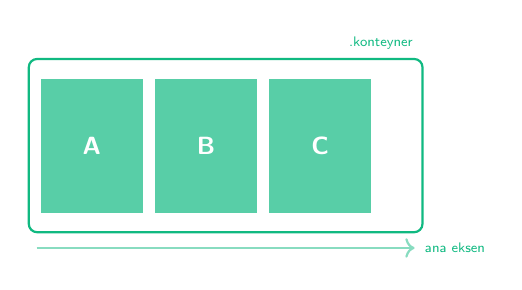
\begin{tikzpicture}
  % konteyner
  \draw[flexcolor, thick, rounded corners=3pt] (0,0.4) rectangle (5.0,2.6);
  \node[flexcolor, font=\sffamily\tiny, above left] at (5.0,2.6) {.konteyner};
  % çocuk elemanlar
  \fill[flexcolor!70] (0.15,0.65) rectangle (1.45,2.35);
  \fill[flexcolor!70] (1.6, 0.65) rectangle (2.9, 2.35);
  \fill[flexcolor!70] (3.05,0.65) rectangle (4.35,2.35);
  \node[white, font=\sffamily\small\bfseries] at (0.8, 1.5) {A};
  \node[white, font=\sffamily\small\bfseries] at (2.25,1.5) {B};
  \node[white, font=\sffamily\small\bfseries] at (3.7, 1.5) {C};
  % yön oku
  \draw[->, thick, flexcolor!50] (0.1,0.2) -- (4.9,0.2)
    node[right, font=\sffamily\tiny, flexcolor] {ana eksen};
\end{tikzpicture}
\end{minipage}
\hfill
\begin{minipage}{0.50\textwidth}
\begin{lstlisting}[style=cssstyle, basicstyle=\ttfamily\footnotesize\color{codefg}]
.konteyner {
  display: flex;
  /* children placed side by side
     and auto-aligned */
}
\end{lstlisting}
\end{minipage}
\end{tcolorbox}

% ----------------------------------------------------------
\newpage
\subsection{Flexbox}

\begin{definebox}[Flexbox Nedir?]
Elemanları tek eksende (satır veya sütun) hizalamak için tasarlanmış
CSS düzen sistemi. Modern arayüzlerin temel taşıdır.
\end{definebox}

\vspace{6pt}

% ---- justify-content karşılaştırması ----
\subsubsection{justify-content — Ana Eksen Hizalaması}

\vspace{4pt}
\noindent
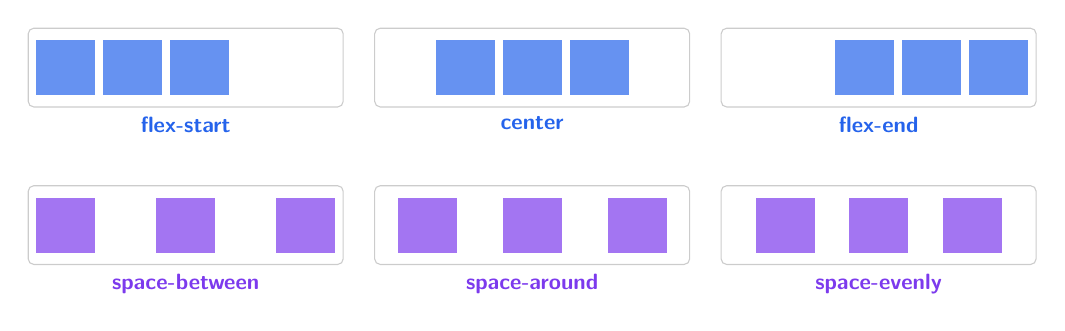
\begin{tikzpicture}
  % flex-start: kutular sol kenara yaslanır (margin=0.10)
  \draw[gray!40, rounded corners=2pt] (0,2.8) rectangle (4.0,3.8);
  \fill[primary!70] (0.10,2.95) rectangle (0.85,3.65);
  \fill[primary!70] (0.95,2.95) rectangle (1.70,3.65);
  \fill[primary!70] (1.80,2.95) rectangle (2.55,3.65);
  \node[font=\sffamily\footnotesize\bfseries, text=primary, below] at (2.0,2.8) {flex-start};

  % center: margin = (4.0 - 3*0.75 - 2*0.10) / 2 = 0.775
  \draw[gray!40, rounded corners=2pt] (4.4,2.8) rectangle (8.4,3.8);
  \fill[primary!70] (5.175,2.95) rectangle (5.925,3.65);
  \fill[primary!70] (6.025,2.95) rectangle (6.775,3.65);
  \fill[primary!70] (6.875,2.95) rectangle (7.625,3.65);
  \node[font=\sffamily\footnotesize\bfseries, text=primary, below] at (6.4,2.8) {center};

  % flex-end: kutular sağ kenara yaslanır (margin=0.10)
  \draw[gray!40, rounded corners=2pt] (8.8,2.8) rectangle (12.8,3.8);
  \fill[primary!70] (10.25,2.95) rectangle (11.00,3.65);
  \fill[primary!70] (11.10,2.95) rectangle (11.85,3.65);
  \fill[primary!70] (11.95,2.95) rectangle (12.70,3.65);
  \node[font=\sffamily\footnotesize\bfseries, text=primary, below] at (10.8,2.8) {flex-end};

  % space-between: uç kutular kenara, aralarında eşit boşluk (0.775)
  \draw[gray!40, rounded corners=2pt] (0,0.8) rectangle (4.0,1.8);
  \fill[secondary!70] (0.10,0.95)  rectangle (0.85,1.65);
  \fill[secondary!70] (1.625,0.95) rectangle (2.375,1.65);
  \fill[secondary!70] (3.15,0.95)  rectangle (3.90,1.65);
  \node[font=\sffamily\footnotesize\bfseries, text=secondary, below] at (2.0,0.8) {space-between};

  % space-around: outer=0.292, inner=0.583  (1.75/6 ve 1.75/3)
  \draw[gray!40, rounded corners=2pt] (4.4,0.8) rectangle (8.4,1.8);
  \fill[secondary!70] (4.692,0.95) rectangle (5.442,1.65);
  \fill[secondary!70] (6.025,0.95) rectangle (6.775,1.65);
  \fill[secondary!70] (7.358,0.95) rectangle (8.108,1.65);
  \node[font=\sffamily\footnotesize\bfseries, text=secondary, below] at (6.4,0.8) {space-around};

  % space-evenly: tüm boşluklar eşit = 1.75/4 = 0.4375
  \draw[gray!40, rounded corners=2pt] (8.8,0.8) rectangle (12.8,1.8);
  \fill[secondary!70] (9.2375,0.95)  rectangle (9.9875,1.65);
  \fill[secondary!70] (10.425,0.95)  rectangle (11.175,1.65);
  \fill[secondary!70] (11.6125,0.95) rectangle (12.3625,1.65);
  \node[font=\sffamily\footnotesize\bfseries, text=secondary, below] at (10.8,0.8) {space-evenly};
\end{tikzpicture}

\vspace{14pt}

% ---- align-items karşılaştırması ----
\subsubsection{align-items — Çapraz Eksen Hizalaması}

\vspace{4pt}
\noindent
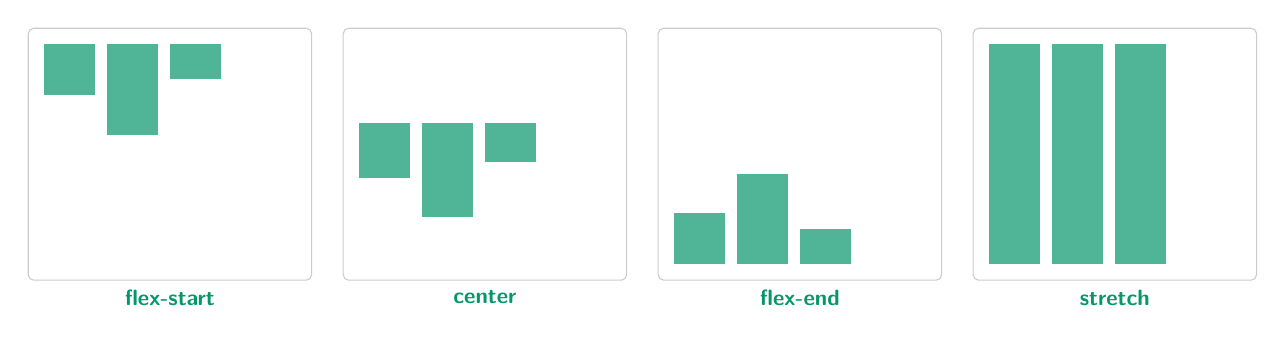
\begin{tikzpicture}
  % flex-start
  \draw[gray!40, rounded corners=2pt] (0,0) rectangle (3.6,3.2);
  \fill[accent!70] (0.2,2.35) rectangle (0.85,3.0);
  \fill[accent!70] (1.0,1.85) rectangle (1.65,3.0);
  \fill[accent!70] (1.8,2.55) rectangle (2.45,3.0);
  \node[font=\sffamily\footnotesize\bfseries, text=accent, below] at (1.8,0) {flex-start};

  % center
  \draw[gray!40, rounded corners=2pt] (4.0,0) rectangle (7.6,3.2);
  \fill[accent!70] (4.2,1.3) rectangle (4.85,2.0);
  \fill[accent!70] (5.0,0.8) rectangle (5.65,2.0);
  \fill[accent!70] (5.8,1.5) rectangle (6.45,2.0);
  \node[font=\sffamily\footnotesize\bfseries, text=accent, below] at (5.8,0) {center};

  % flex-end
  \draw[gray!40, rounded corners=2pt] (8.0,0) rectangle (11.6,3.2);
  \fill[accent!70] (8.2,0.2)  rectangle (8.85,0.85);
  \fill[accent!70] (9.0,0.2)  rectangle (9.65,1.35);
  \fill[accent!70] (9.8,0.2)  rectangle (10.45,0.65);
  \node[font=\sffamily\footnotesize\bfseries, text=accent, below] at (9.8,0) {flex-end};

  % stretch
  \draw[gray!40, rounded corners=2pt] (12.0,0) rectangle (15.6,3.2);
  \fill[accent!70] (12.2,0.2)  rectangle (12.85,3.0);
  \fill[accent!70] (13.0,0.2)  rectangle (13.65,3.0);
  \fill[accent!70] (13.8,0.2)  rectangle (14.45,3.0);
  \node[font=\sffamily\footnotesize\bfseries, text=accent, below] at (13.8,0) {stretch};
\end{tikzpicture}

\vspace{14pt}

\begin{tcolorbox}[enhanced, colback=codebg, colframe=gray!30,
    colbacktitle=primary!85!black, coltitle=white, arc=4pt,
    title={\sffamily\bfseries\small Flexbox Örnekleri}]
\begin{lstlisting}[style=cssstyle]
/* Center both horizontally and vertically */
.container {
  display: flex;
  justify-content: center;  /* horizontal (main axis)  */
  align-items: center;      /* vertical (cross axis)   */
  height: 100vh;
}

/* Spread cards side by side */
.card-list {
  display: flex;
  justify-content: space-between;
  gap: 16px;
  flex-wrap: wrap;          /* wrap to next line */
}

/* Navbar: logo left, links right */
.navbar {
  display: flex;
  justify-content: space-between;
  align-items: center;
  padding: 0 24px;
}
\end{lstlisting}
\end{tcolorbox}

% ============================================================
\newpage
\section{\faHammer\ Pratik: Card UI Oluşturma}
\timebadge{70--90 dakika}

\begin{practicebox}[\faTasks\ Pratik Hedef]
Flexbox kullanarak üç kart içeren bir ürün listesi sayfası oluşturun.
Kartlar:
\begin{itemize}
  \item Görsel (placeholder), başlık, açıklama ve buton içerecek
  \item Yan yana sıralanacak
  \item Hover'da hafif gölgelenecek
\end{itemize}
\end{practicebox}

\vspace{8pt}
\textbf{Adım 1 --- HTML Yapısı}

\begin{tcolorbox}[enhanced, colback=codebg, colframe=gray!30,
    colbacktitle=primary!85!black, coltitle=white, arc=4pt,
    title={\sffamily\bfseries\small index.html}]
\begin{lstlisting}[style=htmlstyle]
<!DOCTYPE html>
<html lang="tr">
<head>
  <meta charset="UTF-8" />
  <title>Product Cards</title>
  <link rel="stylesheet" href="style.css" />
</head>
<body>

  <header class="site-header">
    <h1>Our Products</h1>
  </header>

  <main class="card-grid">

    <!-- Each card repeats the same structure -->
    <article class="card">
      <img src="https://via.placeholder.com/300x180" alt="Product 1" />
      <div class="card-body">
        <h2 class="card-title">Product Title</h2>
        <p class="card-desc">Short product description.</p>
        <button class="btn">View</button>
      </div>
    </article>

    <!-- <article class="card"> ... </article>  x2 more -->

  </main>

</body>
</html>
\end{lstlisting}
\end{tcolorbox}

\vspace{8pt}
\textbf{Adım 2 --- CSS Stilleri}

\begin{tcolorbox}[enhanced, colback=codebg, colframe=gray!30,
    colbacktitle=primary!85!black, coltitle=white, arc=4pt,
    title={\sffamily\bfseries\small style.css}]
\begin{lstlisting}[style=cssstyle]
* { box-sizing: border-box; margin: 0; padding: 0; }

body { font-family: sans-serif; background: #f1f5f9; color: #1e293b; }

.site-header {
  background: #2563eb;
  color: white;
  padding: 24px;
  text-align: center;
}

.card-grid {
  display: flex;
  justify-content: center;
  gap: 24px;
  flex-wrap: wrap;
  padding: 40px 24px;
}

.card {
  background: white;
  border-radius: 12px;
  box-shadow: 0 2px 8px rgba(0,0,0,0.08);
  width: 300px;
  overflow: hidden;
  display: flex;
  flex-direction: column;
  transition: box-shadow 0.2s ease, transform 0.2s ease;
}

.card:hover {
  box-shadow: 0 8px 24px rgba(0,0,0,0.15);
  transform: translateY(-4px);
}

.card img { width: 100%; display: block; }

.card-body {
  padding: 20px;
  display: flex;
  flex-direction: column;
  gap: 12px;
  flex: 1;
}

.card-title { font-size: 1.1rem; font-weight: 700; }
.card-desc  { font-size: 0.9rem; color: #64748b; flex: 1; }

.btn {
  background: #2563eb;
  color: white;
  border: none;
  border-radius: 8px;
  padding: 10px 20px;
  font-weight: 600;
  cursor: pointer;
}

.btn:hover { background: #1d4ed8; }
\end{lstlisting}
\end{tcolorbox}

\vspace{12pt}
\textbf{Tarayıcı Çıktısı}

\vspace{6pt}
\begin{center}
  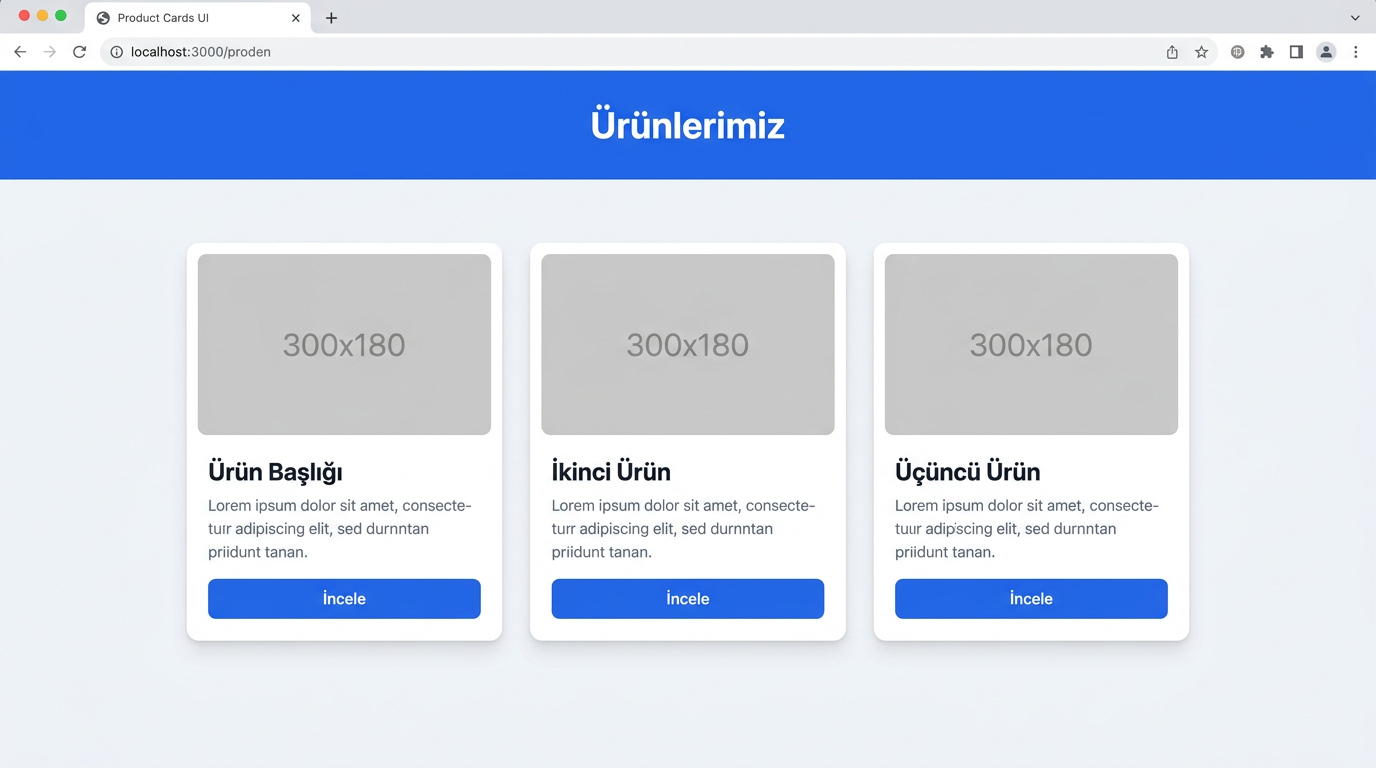
\includegraphics[width=0.90\textwidth]{card-ui-output.png}
  \captionof*{figure}{\small\sffamily\color{gray}
    Pratik kodunun tarayıcıdaki görünümü: üç kart yan yana, hover efektiyle}
\end{center}

% ============================================================
\newpage
\section{\faCheckCircle\ Özet ve Sonraki Session}

\subsection{Bu Session'da Öğrendiklerimiz}

\begin{tcolorbox}[enhanced, colback=lightbg, colframe=gray!30, arc=4pt]
\begin{itemize}
  \item[\color{accent}\faCheck] Web nasıl çalışır: Browser--Server, HTTP, Request/Response
  \item[\color{accent}\faCheck] HTML iskelet yapısı: \texttt{<!DOCTYPE>}, \texttt{<head>}, \texttt{<body>}
  \item[\color{accent}\faCheck] Semantic etiketler: \texttt{header, nav, main, section, footer}
  \item[\color{accent}\faCheck] Form öğeleri: \texttt{input, label, button}
  \item[\color{accent}\faCheck] CSS Box Model: content / padding / border / margin
  \item[\color{accent}\faCheck] \texttt{display}: block, inline, flex farkları
  \item[\color{accent}\faCheck] Flexbox: \texttt{justify-content}, \texttt{align-items}, \texttt{gap}, \texttt{flex-wrap}
  \item[\color{accent}\faCheck] Pratik: Card UI --- gerçek bir bileşen sıfırdan yazdık
\end{itemize}
\end{tcolorbox}

\vspace{6pt}

\subsection{Sıkça Sorulan Sorular}

\begin{warningbox}[\faQuestionCircle\ SSS]
\textbf{S: \texttt{div} ile \texttt{section} ne zaman kullanılır?}\\
C: \texttt{<section>} tematik bir içerik grubuysa, \texttt{<div>} yalnızca
stil/layout için bir kapsayıcıysa kullanılır.

\vspace{6pt}
\textbf{S: \texttt{padding} mi \texttt{margin} mi?}\\
C: Elemanın \textit{iç} boşluğu için \texttt{padding}, dış boşluğu için \texttt{margin}.

\vspace{6pt}
\textbf{S: Flexbox mu Grid mi?}\\
C: Tek boyutlu (satır veya sütun) düzen için Flexbox, iki boyutlu
(satır \textit{ve} sütun) için CSS Grid kullanılır.
\end{warningbox}

\vspace{6pt}

\subsection{Sonraki Session --- Session 2: Modern JavaScript}

\begin{infobox}[\faArrowRight\ Session 2 (29 Nisan Çarşamba)]
React öncesi için ihtiyaç duyacağımız temel JavaScript konuları:
\begin{itemize}
  \item \textbf{let / const}, arrow functions, template literals
  \item \textbf{Destructuring}, spread/rest operatörleri
  \item \textbf{Array methods}: \texttt{map}, \texttt{filter}, \texttt{reduce}
  \item \textbf{async/await} ve \texttt{fetch} API ile veri çekme
\end{itemize}
\end{infobox}

\vspace{16pt}
\begin{center}
  \color{gray}\sffamily\small
  Front-end + Next.js Eğitimi \quad|\quad Session 1 / 8 \quad|\quad 27 Nisan 2026
\end{center}

\end{document}
